\graphicspath{{main/design/hardware/graphics/}}

\subsection{Development Test Harness} \label{sec:testHarness}

Similar to the development cards, dedicated and isolated hardware was required for the test harness. This was to perform validation against the developed software to ensure the real-time requirements were maintained. Through the harness, an example control loop implementation could be simulated to ensure all deadlines are met during a live software update.

\begin{figure}[ht]
    \centering
    \begin{tikzpicture}  
        \node[block] (gen) {Signal\\Generator}; 
        \node[block, right=2cm of gen] (sw) {Software\\Infrastructure};
        \node[block, right=2cm of sw] (rcv) {Signal\\Receiver};  
        
        \node[block, text width=12cm, minimum height=1cm, below=1cm of sw] (har) {Harness}; 
        \node[block, minimum height=1cm, below=1cm of har] (ana) {Analyser};  

        \draw[->,thick] (gen) edge (sw);
        \draw[->,thick] (sw) edge (rcv);

        \draw[->,thick] (gen.south) edge ([xshift=-5.3cm]har.north);
        \draw[->,thick] (rcv.south) edge ([xshift=5.3cm]har.north);

        \draw[->,thick] (har) edge (ana);
    \end{tikzpicture}  
    \caption[Test harness design]
    {Test harness design}
    \label{fig:testHarnessDesign}
\end{figure}

% WRONG TENSE
\autoref{fig:testHarnessDesign} contains a signal generator, this randomly produces a signal and outputs a packet. These packets are ingested by the software infrastructure where processing occurs. An output packet is subsequently generated (mirroring the input) and sent to a signal receiver, which captures this packet.

The signal generator and receiver output their current state over discrete digital signals so that a logic analyser can record the state of the system over time. Specifically the states can be compared to measure the complete system latency during standard operation and software update. If the generator and receiver produce additional reference clock signals, the logic analyser can more closely calculate the software infrastructure induced latency.

The theoretical logic analyser output is displayed in \autoref{fig:testHarnessCapture}. The latency between generate and receive is shown on the latency channel.

\begin{figure}[ht]
    \centering
    \begin{tikztimingtable}[%
        timing/dslope=0.1,
        timing/.style={x=2ex,y=2ex},
        x=2ex,
        timing/rowdist=3ex,
    ]
        \busref{Generator Clock} & 2l 10{4c} \\
        \busref{Reciever Clock } & 11{4c} \\
        \busref{Generator Signal} & 6h 16l 16h 4l \\
        \busref{Reciever Signal} & 8h 16l 16h 4l \\

        \busref{Latency} & 6l D{} 14l  D{} 14l D{} 2l \\
        \extracode
            \begin{pgfonlayer}{background}
            \begin{scope}[semitransparent ,semithick]
                \vertlines[darkgray,dotted]{0.5,1.0 ,...,20.0}
            \end{scope}
        \end{pgfonlayer}
    \end{tikztimingtable}
    \caption[Test harness capture]
    {Test harness capture}
    \label{fig:testHarnessCapture}
\end{figure}

The generator, receiver and logic analyser were all implemented using the RP2040 microprocessor from Raspberry Pi for hardware simplification. The two controllers that performed message communication used the W5500 chip to send UDP packets over ethernet, this integrated nicely with software infrastructure. The co-processor offloads the complex ethernet drivers and communicates to the main processor over SPI. The embedded network switch selected to connect the different elements of the test harness with the development cards was the SwitchBlox 'Small Ethernet Switch'.

\autoref{fig:TestHardwareFrameMount} displays the frame mount designed in Fusion 360 and 3D printed, to hold the components together in a single package. Harness is shown assembled in \autoref{fig:TestHarnessHardware}.

\begin{figure}[ht]
    \centering
    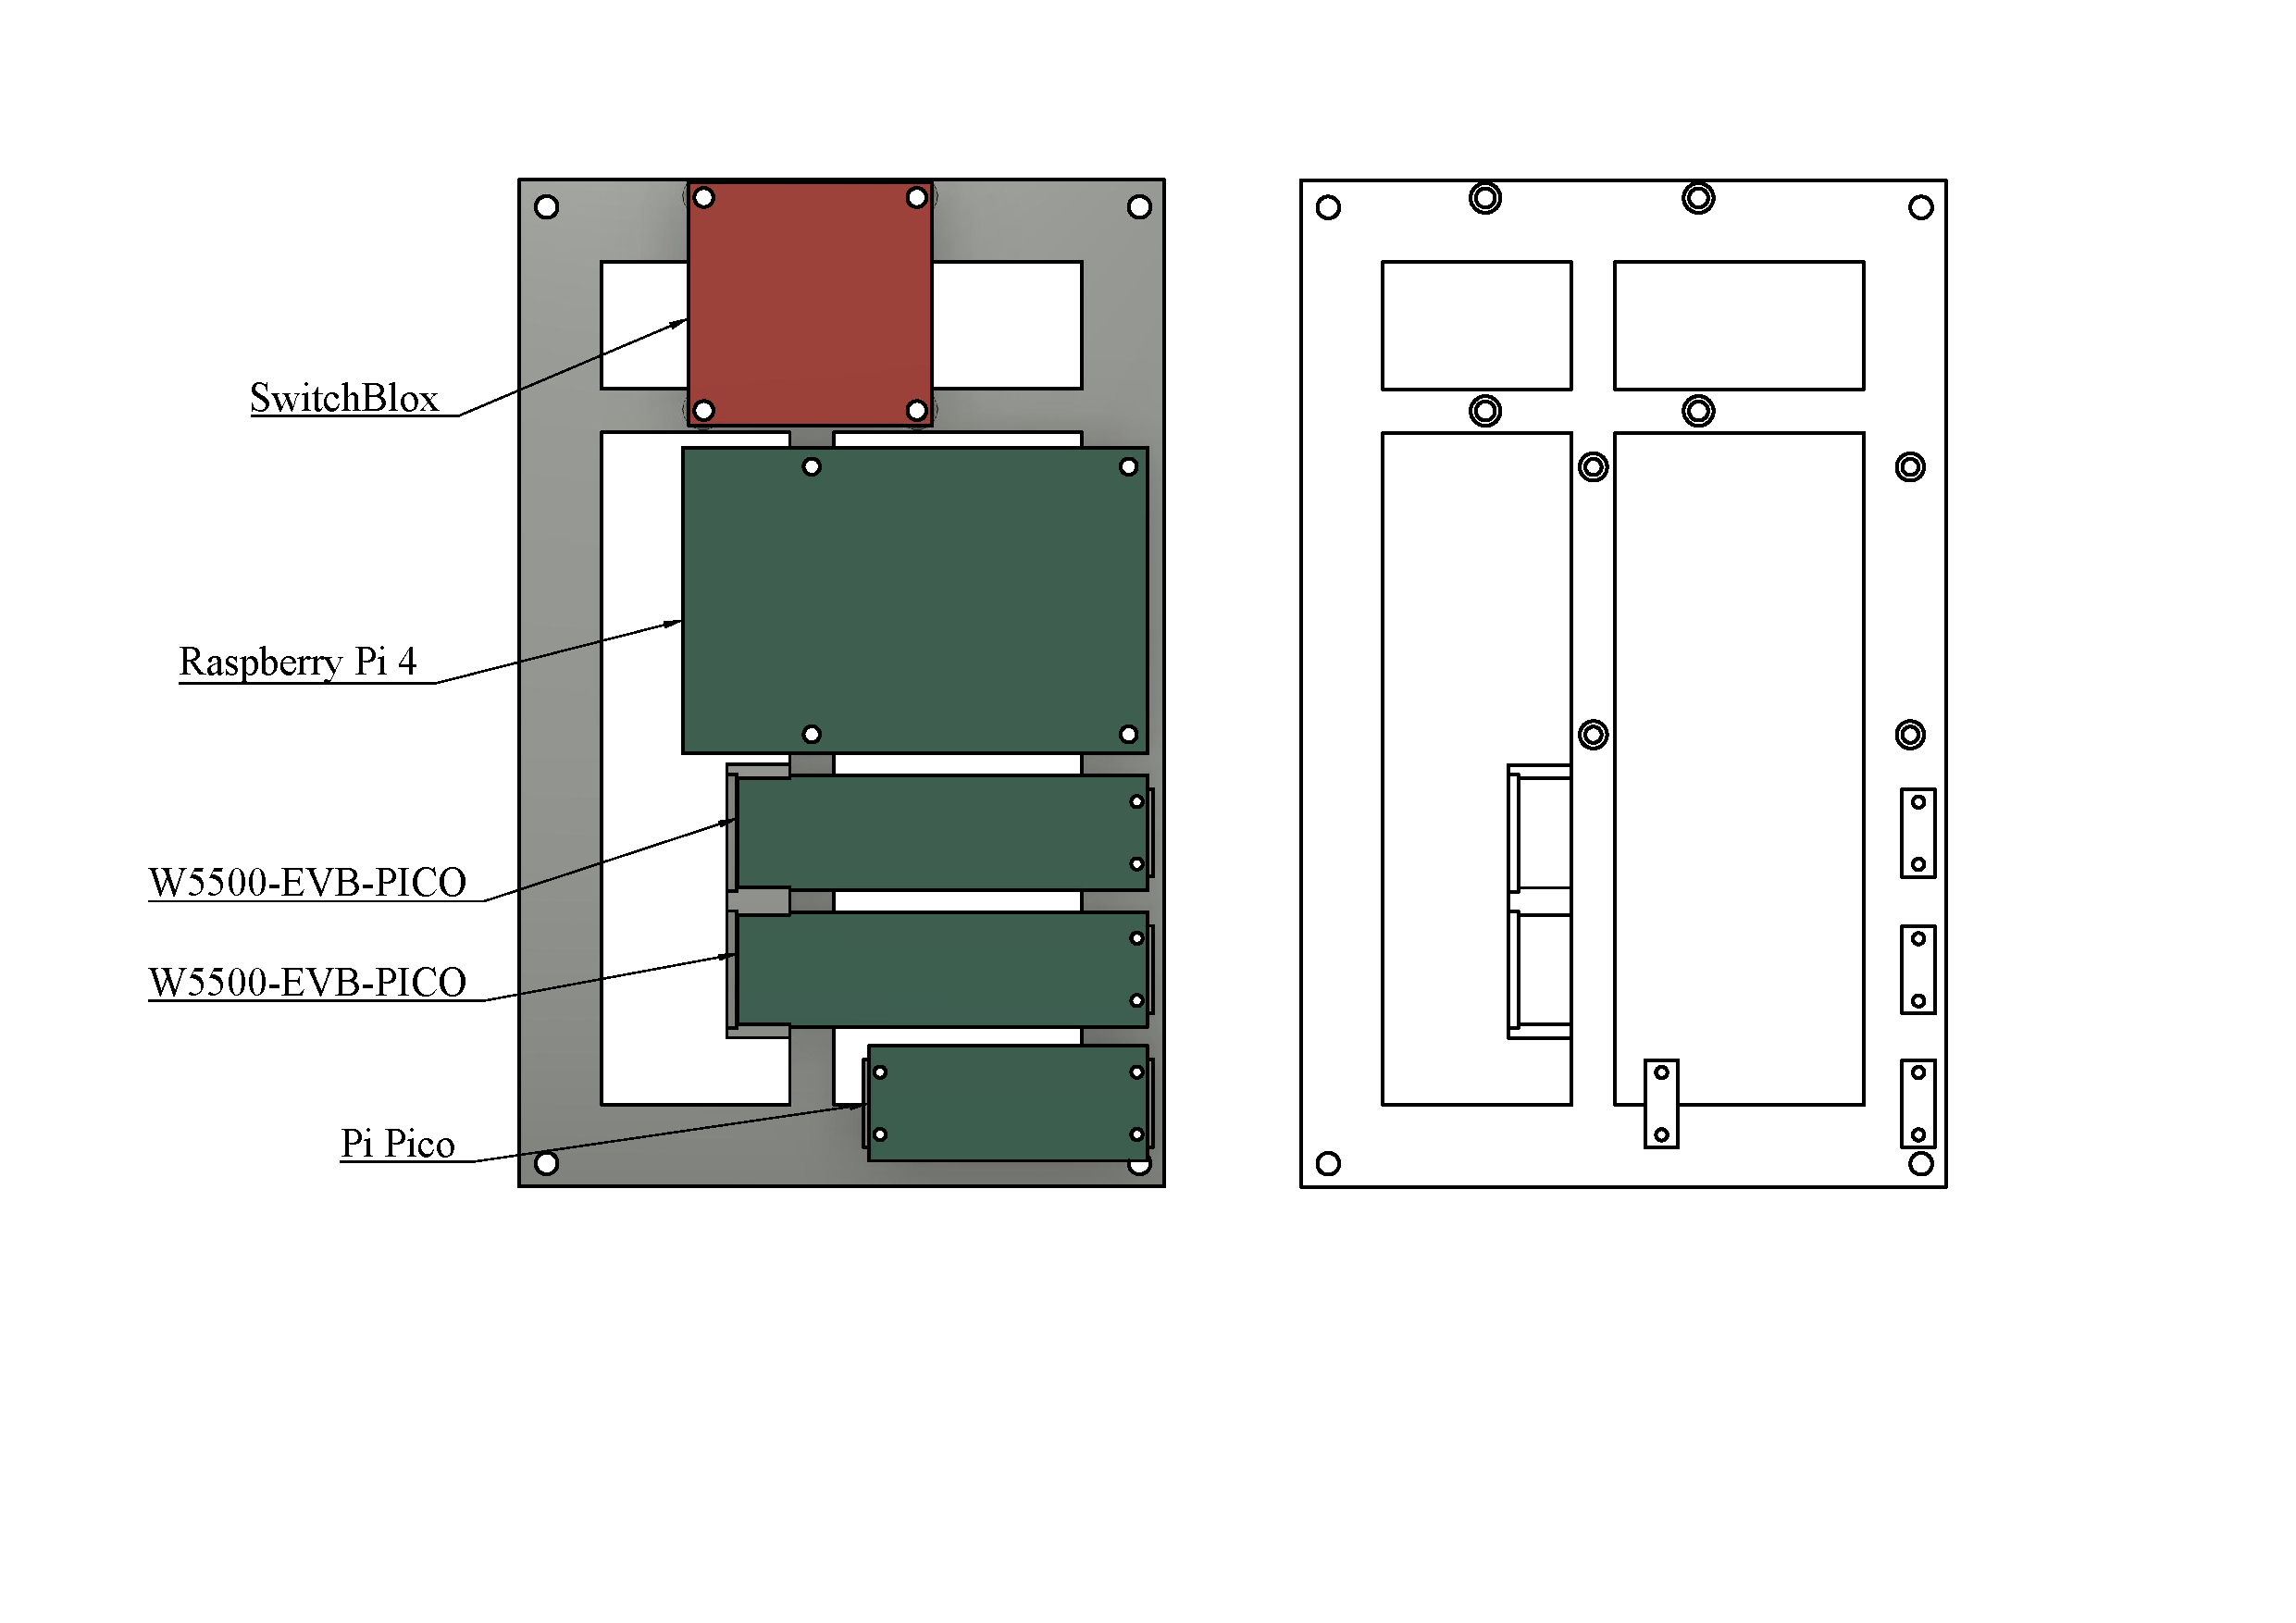
\includegraphics[width=\textwidth, clip, trim=0.5cm 7cm 0.5cm 2cm]{TestHardwareFrameMount.pdf}
    \caption[Test harness hardware frame mount design]
    {Test harness hardware frame mount design}
    \label{fig:TestHardwareFrameMount}
\end{figure}

\begin{figure}[ht]
    \centering
    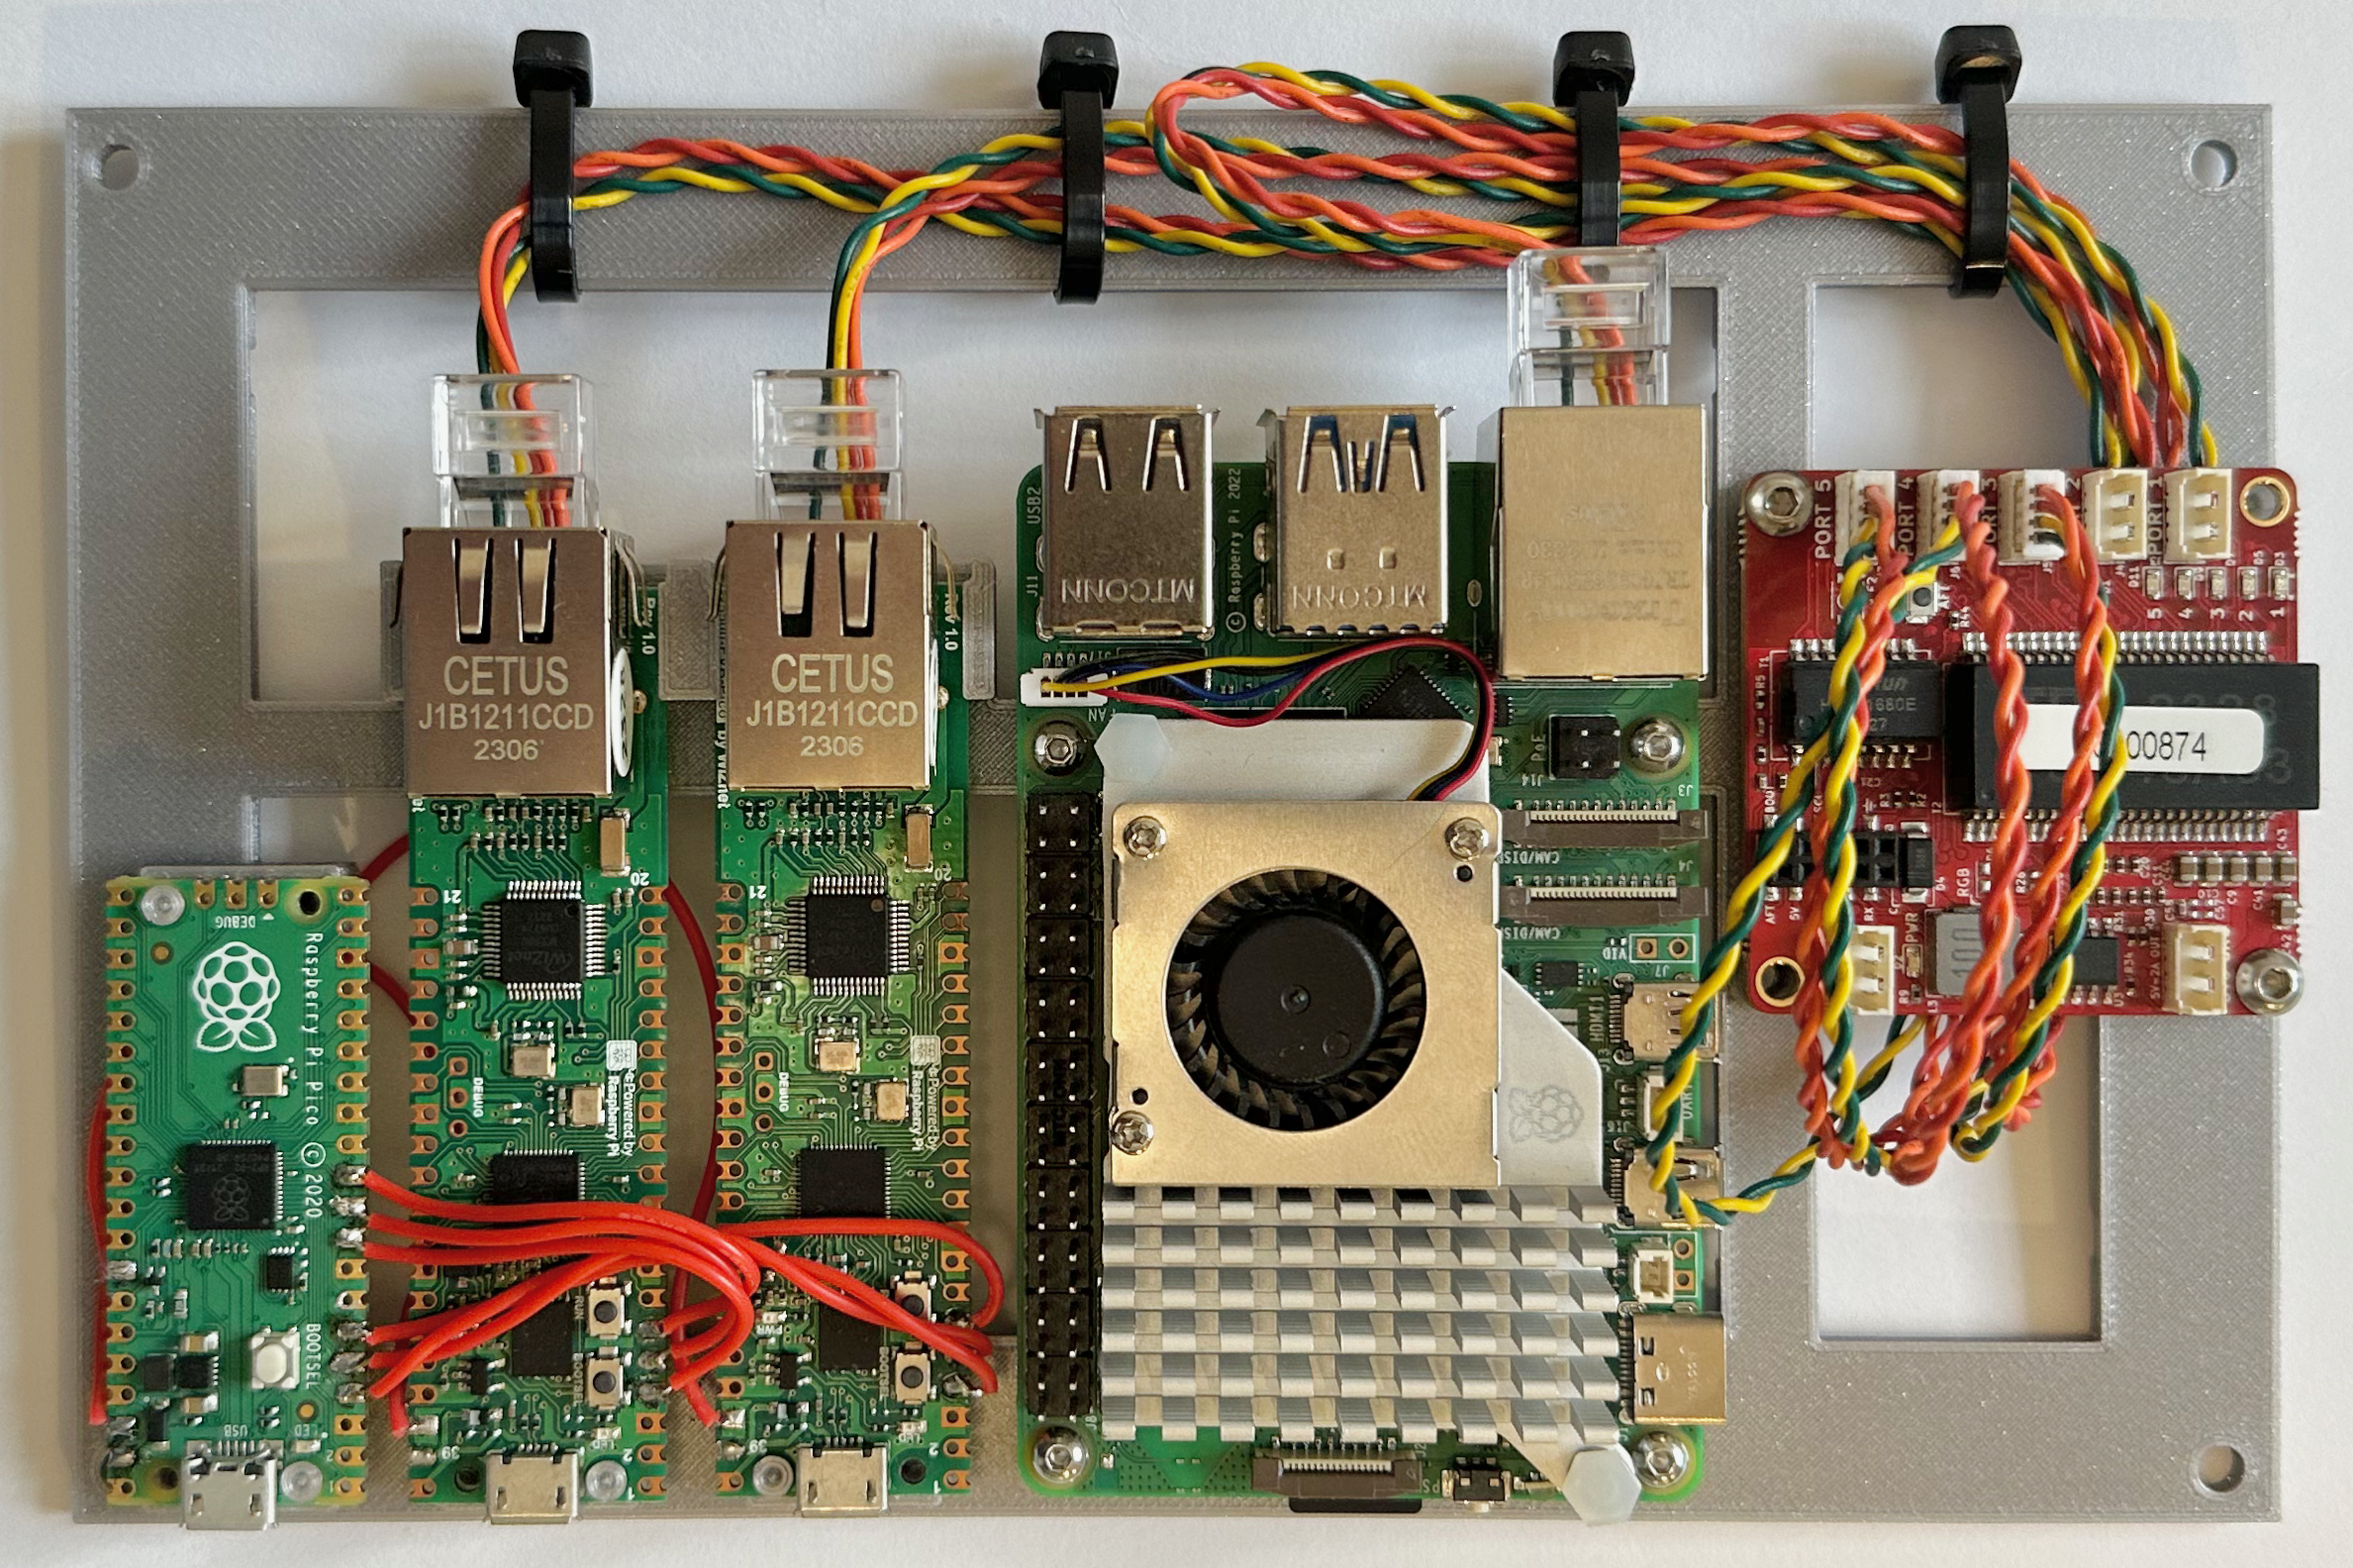
\includegraphics[width=10cm, clip]{TestHarnessHardware}
    \caption[Test harness hardware assembled]
    {Test harness hardware assembled}
    \label{fig:TestHarnessHardware}
\end{figure}

\clearpage


\begin{table}[ht]
    \centering
    \begin{tabular}{ c|ccc } 
        \hline
        Name & Manufacturer & Quantity & Task \\ 
        \hline
        \href{https://www.raspberrypi.com/products/raspberry-pi-4-model-b/}{Raspberry Pi 4} & Raspberry Pi & 1 & Boot Server \\ 
        \href{https://www.raspberrypi.com/products/raspberry-pi-pico/}{Raspberry Pi Pico} & Raspberry Pi & 3 & Test Hardware \\ 
        \href{https://botblox.io/products/small-ethernet-switch}{Small Ethernet Switch} & SwitchBlox & 1 & Network Switch \\ 
    \end{tabular}
    \caption[Development hardware bill-of-materials]
    {Development hardware bill-of-materials}
    \label{tbl:TestHarnessHardwareBOM}
\end{table}



The chosen logic analyser software was PulseView as it is open-source and supports many different logic analyser devices \autocite{pulseviewPulseViewSigrok}. Boards which use the RP2040 microprocessor (Pi Pico) can use the ULA logic analyser firmware \autocite{domnikovDotcypressUla2024}.

When flashed, the Pi Pico can capture the status of 16 input channels at specified frequencies. An example capture is shown in \autoref{fig:testHarnessPluseViewCapture}.

\begin{figure}[ht]
    \centering
    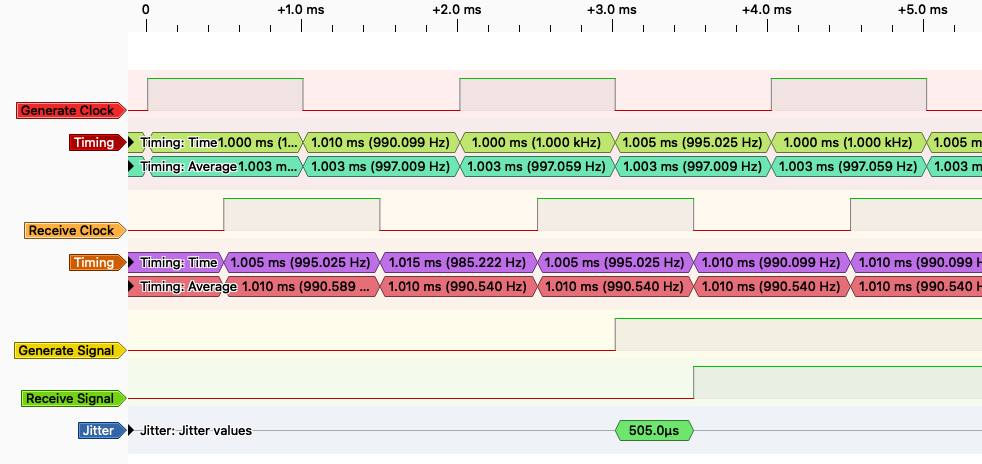
\includegraphics[width=\textwidth]{testHarnessPluseViewCapture.png}
    \caption[Test harness PluseView capture]
    {Test harness PluseView capture}
    \label{fig:testHarnessPluseViewCapture}
\end{figure}